\documentclass[border=10pt,tikz]{standalone}
\usepackage[utf8]{inputenc}
\usepackage{tikz}
\usetikzlibrary{arrows.meta, positioning}
\usepackage{xcolor}
\usepackage{amsmath}

\definecolor{cRed}{HTML}{C0392B}
\definecolor{cAmber}{HTML}{F39C12}
\definecolor{cGray}{HTML}{7F8C8D}

\begin{document}
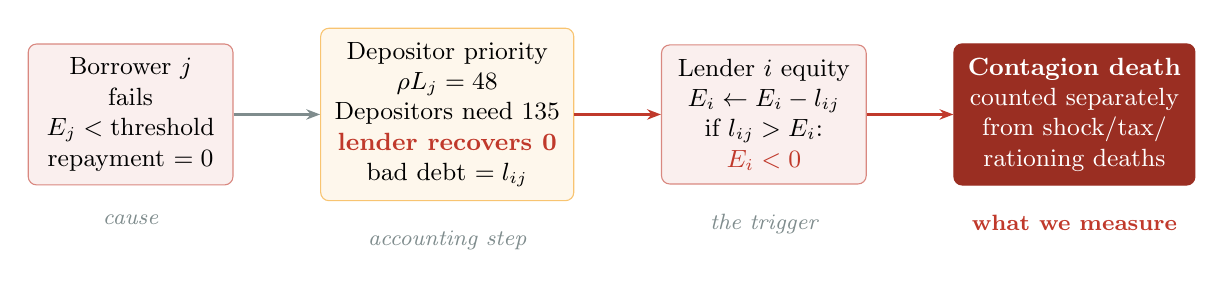
\begin{tikzpicture}[
  node distance=0.7cm and 1.1cm,
  cbox/.style={rectangle, rounded corners=3pt, draw, minimum width=2.6cm,
              minimum height=1.5cm, align=center, font=\small,
              inner sep=5pt},
  redbox/.style={cbox, fill=cRed!8, draw=cRed!60},
  amberbox/.style={cbox, fill=cAmber!8, draw=cAmber!60},
  darkbox/.style={cbox, fill=cRed!80!black, draw=cRed!80!black,
                  text=white},
  arr/.style={-{Stealth[length=5pt]}, line width=0.9pt, color=cGray},
  redarr/.style={-{Stealth[length=5pt]}, line width=1.1pt, color=cRed},
]

\node[redbox] (fail) {Borrower $j$\\fails\\$E_j < \text{threshold}$\\repayment $= 0$};

\node[amberbox, right=of fail] (waterfall)
  {Depositor priority\\$\rho L_j = 48$\\Depositors need 135\\
   \textcolor{cRed}{\textbf{lender recovers 0}}\\bad debt $= l_{ij}$};

\node[redbox, right=of waterfall] (equity)
  {Lender $i$ equity\\$E_i \leftarrow E_i - l_{ij}$\\if $l_{ij} > E_i$:\\
   \textcolor{cRed}{\textbf{$E_i < 0$}}};

\node[darkbox, right=of equity] (death)
  {\textbf{Contagion death}\\counted separately\\from shock/tax/\\rationing deaths};

\draw[arr]    (fail)      -- (waterfall);
\draw[redarr] (waterfall) -- (equity);
\draw[redarr] (equity)    -- (death);

\node[font=\footnotesize\itshape, color=cGray, below=0.25cm of fail]
  {cause};
\node[font=\footnotesize\itshape, color=cGray, below=0.25cm of waterfall]
  {accounting step};
\node[font=\footnotesize\itshape, color=cGray, below=0.25cm of equity]
  {the trigger};
\node[font=\footnotesize\color{cRed}, below=0.25cm of death]
  {\textbf{what we measure}};

\end{tikzpicture}
\end{document}
